% PVLDB research-track paper skeleton.
% Template: PVLDB uses acmart (sigconf, nonacm) with the VLDB header blocks below.
% Before submission, replace the preamble and blocks with the current official template
% from https://vldb.org/pvldb/ and check the current call for papers for the page limit
% (research papers: 12 pages plus references) and the anonymity rules.
%
% Build: tectonic main.tex   (or: latexmk -pdf main.tex)
% Figures are read from ../results/figures/, so regenerate them there.
% Every number below comes from results/FULL-RESULTS.md, results/RELATED-WORK.md or a
% script named in a comment, all computed from archived runs. Open items are marked \todo{}.

\documentclass[sigconf, nonacm]{acmart}

\usepackage{booktabs}
\usepackage{xcolor}
\usepackage{tikz}
\usetikzlibrary{positioning,fit,arrows.meta}
\graphicspath{{../results/figures/}}

\newcommand{\todo}[1]{\textcolor{red}{[TODO: #1]}}
\newcommand{\sys}{GPU offload}
\newcommand{\takeaway}[1]{\par\smallskip\noindent\fbox{\parbox{\dimexpr\columnwidth-2\fboxsep-2\fboxrule}{\small\textbf{Takeaway.} #1}}\par\smallskip}

%%% VLDB block start %%%
\newcommand\vldbdoi{XX.XX/XXX.XX}
\newcommand\vldbpages{XXX-XXX}
\newcommand\vldbvolume{XX}
\newcommand\vldbissue{X}
\newcommand\vldbyear{2027}
\newcommand\vldbauthors{\authors}
\newcommand\vldbtitle{\shorttitle}
% Leave empty for a double-blind submission; the repository URL identifies the authors.
\newcommand\vldbavailabilityurl{}
\newcommand\vldbpagestyle{plain}
%%% VLDB block end %%%

\begin{document}

% Title options:
%   One GPU, Many Databases: Whole-Compaction Offload as a Shared Service for RocksDB
%   Compression Is What Is Left: Whole-Compaction GPU Offload, Shared Across Databases
\title{One GPU, Many Databases: Whole-Compaction Offload as a Shared Service for RocksDB}

\author{\todo{Authors}}
\affiliation{\institution{\todo{Institution}}\city{\todo{City}}\country{\todo{Country}}}

\begin{abstract}
Compaction is the largest CPU cost of a write-heavy LSM-tree store. Earlier GPU and FPGA
designs move sorting, merging and block building off the CPU, but leave block compression
behind. Rebuilt stage by stage inside RocksDB~11.8 and measured on one machine, the stronger
family still uses 49\% of RocksDB's compaction CPU with LZ4 and 69\% with ZSTD. We offload all of compaction's per-byte work,
compression included, while RocksDB keeps its own file boundaries, index, filters and
installation, and we check the results against unmodified RocksDB. One GPU then does the
compaction work of 15--18 cores, and when compaction is the CPU bottleneck the database
accepts 1.5--1.8$\times$ more writes. But one database keeps a GPU only 19\% busy, and a GPU
dedicated to one database costs 1.39$\times$ as much per GiB/s of compaction as the cores it
replaces. We therefore run GPU compaction as a shared service that databases reach over
shared memory, RDMA or TCP. Eight databases of 4 cores on another machine each get
1.99$\times$ RocksDB's writes on the same cores over 5-minute runs, counting the compaction
left when writing stops, with no compaction falling back to the CPU; the GPU is then 98\% busy. At that load the
service costs 5\% more per write than RocksDB at the measured card's cloud price and breaks
even at \$2.73 an hour. The service does not yet isolate tenants, and throughput is unchanged
when a drive is the bottleneck. Unless stated otherwise, results are for batched writes with
the write-ahead log off and data in memory.
\end{abstract}

\maketitle

%%% VLDB block start %%%
\pagestyle{\vldbpagestyle}
\begingroup\small\noindent\raggedright\textbf{PVLDB Reference Format:}\\
\vldbauthors. \vldbtitle. PVLDB, \vldbvolume(\vldbissue): \vldbpages, \vldbyear.\\
\href{https://doi.org/\vldbdoi}{doi:\vldbdoi}
\endgroup
\begingroup
\renewcommand\thefootnote{}\footnote{\noindent
This work is licensed under the Creative Commons BY-NC-ND 4.0 International License. Visit
\url{https://creativecommons.org/licenses/by-nc-nd/4.0/} to view a copy of this license.
For any use beyond those covered by this license, obtain permission by emailing
\href{mailto:info@vldb.org}{info@vldb.org}. Copyright is held by the owner/author(s).
Publication rights licensed to the VLDB Endowment. \\
\raggedright Proceedings of the VLDB Endowment, Vol. \vldbvolume, No. \vldbissue\ %
ISSN 2150-8097. \\
\href{https://doi.org/\vldbdoi}{doi:\vldbdoi} \\
}\addtocounter{footnote}{-1}\endgroup
%%% VLDB block end %%%

%%% VLDB block start %%%
\ifdefempty{\vldbavailabilityurl}{}{
\vspace{.3cm}
\begingroup\small\noindent\raggedright\textbf{PVLDB Artifact Availability:}\\
The source code, data, and/or other artifacts have been made available at
\url{\vldbavailabilityurl}.
\endgroup
}
%%% VLDB block end %%%

% ------------------------------------------------------------------------------------------
\section{Introduction}
\label{sec:intro}

LSM-trees~\cite{oneil1996lsm} accept writes into memory and keep data sorted on storage by
merging files in the background. In RocksDB~\cite{dong2021rocksdb} this merging, compaction,
is the largest CPU cost of a write-heavy database: with 128-byte values it takes
3.5--5.5\,\textmu s of CPU per write, more than accepting the write itself (2.3\,\textmu s,
Figure~\ref{fig:cpu-split}). RocksDB's developers report that its optimisation priority has
moved from write amplification, to space amplification, to CPU~\cite{dong2021rocksdb}. When
compaction falls behind, RocksDB slows its writers~\cite{silk2019,adoc2023}, and the work it
postpones still has to be done.

Accelerators have been applied to compaction for six years. GPU
designs~\cite{luda2020,glsm2024,zhou2024msst,gpcomp2025,gclcomp2025,gparakv2025} and an
FPGA design~\cite{fpga2020} take the sort and merge off the CPU, and some also build blocks,
compute checksums~\cite{luda2020} or move data from the SSD to the GPU
directly~\cite{gpcomp2025}. Each reports its gain on its own store (LevelDB, X-Engine or a
key-value-separated store) and its own hardware, so the results cannot be compared with each
other or with RocksDB, and it is not known which part of compaction still costs CPU after
offload.

\paragraph{The codec is what is left.} We rebuilt both families of earlier designs inside
RocksDB~11.8 and measured them on one machine against the same inputs
(Section~\ref{sec:motivation}). The stronger family still leaves 49\% of RocksDB's
compaction CPU on the CPU with LZ4 and 69\% with ZSTD. With compression turned off, the same
rebuild uses the same CPU as a full offload: what earlier designs leave behind is block
compression and decompression. None of the designs we could examine offloads it; LUDA lists
it as future work~\cite{luda2020}.

\paragraph{One database does not need a whole GPU.} With the codec on the GPU too, one GPU
does the compaction work of 15--18 RocksDB cores. A database of 4 cores writing as fast as it
can keeps that GPU busy only 19\% of the time, and a GPU dedicated to one database costs
1.39$\times$ as much per GiB/s of compaction as the cores it replaces
(Section~\ref{sec:motivation-idle}). GPU compaction can only approach the cost of
CPU cores as a shared resource, as CaaS-LSM made CPU compaction a
service~\cite{caaslsm2024}.

\paragraph{Our approach.} We offload all of compaction's per-byte work (decompression,
merging, block building, compression, checksums and Bloom-filter hashing; we call this
\emph{whole-compaction offload}) while RocksDB keeps every decision that shapes the tree:
where output files end, the index, filter sizing, metadata and installation
(Section~\ref{sec:offload}). The interface between the two is a self-contained request (the
input blocks) and a reply (finished blocks), so the GPU needs no access to the database's
files or tree. That is what lets one GPU serve many databases. We run this offload as a shared service: one
process owns the GPU, schedules the compactions of many databases on a few GPU engines,
re-queues jobs that run out of GPU memory instead of failing them, and is reached over shared
memory, RDMA or TCP (Section~\ref{sec:service}). In every single-compaction run, every stored
version and 200{,}000 lookups match unmodified RocksDB; every whole-database run verifies
every key; and any job the GPU cannot take runs on RocksDB's
own code.

\begin{figure}[t]
  \centering
  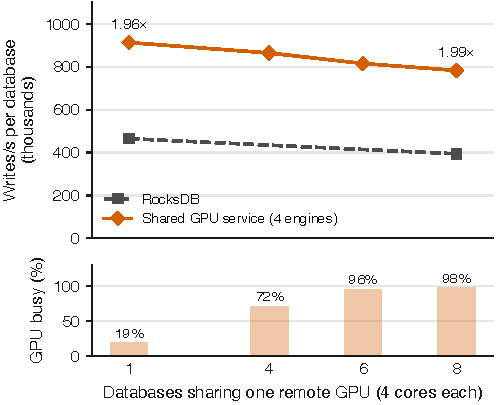
\includegraphics[width=0.92\columnwidth]{fig48_capacity_m5.pdf}
  \caption{Databases of 4 cores on one machine sharing one GPU on another through the
  compaction service over RDMA, against RocksDB on the same cores. Top: writes per second
  per database, counted to the end of the compaction left when writing stops. Bottom: GPU
  utilisation during writing. Median of 3 runs; no compaction fell back to the CPU.}
  \label{fig:capacity}
\end{figure}

\paragraph{Results.} When compaction is the CPU bottleneck, the database accepts
1.5--1.8$\times$ more writes, CPU per write roughly halves, and 99.9th-percentile write
latency under load falls 3.8--9.6$\times$. When other programs take 40--80\% of the
database's cores, the gain grows to 2.2--2.5$\times$. Read-heavy YCSB workloads are
unchanged. Eight databases on one machine sharing a GPU on another each get 1.99$\times$
RocksDB's writes on the same cores over 5-minute runs, counting the compaction left at the
end, with the GPU 98\% busy (Figure~\ref{fig:capacity}). At the measured GPU price this costs
5\% more per write than RocksDB; it is cheaper below \$2.73 an hour. We
state the regime of every result: the headline runs keep data in memory with the write-ahead
log off and writes in batches of 100, which makes compaction the bottleneck. When a drive is
the bottleneck, throughput is unchanged and only the CPU saving remains.

\paragraph{Contributions.}
\begin{itemize}
  \item A same-harness evaluation of earlier GPU and FPGA compaction designs, rebuilt in
        RocksDB under rules registered before the runs. It identifies the codec as what they
        leave on the CPU (Section~\ref{sec:motivation}).
  \item Whole-compaction GPU offload inside production RocksDB, compression included, checked
        against unmodified RocksDB on every compaction: compaction 8.0--11.7$\times$ faster
        with 8.8--15.5$\times$ less CPU, and 1.5--1.8$\times$ more writes for the whole
        database (Sections~\ref{sec:offload}, \ref{sec:eval-compaction},
        \ref{sec:eval-db}).
  \item A shared GPU compaction service with tenant scheduling and out-of-memory re-queueing,
        reached over shared memory, RDMA or TCP. Eight remote databases each get
        1.99$\times$ RocksDB's writes, with no CPU fallback in 84 registered service runs
        (Sections~\ref{sec:service}, \ref{sec:eval-sharing}).
  \item A cost analysis: GPU compaction is cheaper per GiB/s of compaction than CPU cores
        only when the GPU is shared close to its capacity, and near parity per write. We give break-even GPU prices so that readers can
        apply their own (Section~\ref{sec:eval-cost}).
\end{itemize}
Every hypothesis and threshold was registered before its runs, and we report those that were
not met (Section~\ref{sec:limits}).

% ------------------------------------------------------------------------------------------
\section{Background and Motivation}
\label{sec:background}

\paragraph{Compaction in RocksDB.} RocksDB keeps data in levels of sorted files. Level 0
holds flushed memtables, whose key ranges overlap; each deeper level is one sorted run about
ten times larger than the one above. A compaction merges files of adjacent levels in five
steps: (1)~read and decompress the input data blocks; (2)~merge them by key, dropping versions
hidden by newer ones and deletions that no longer shadow anything; (3)~pack the surviving
entries into data blocks; (4)~compress and checksum each block and hash its keys for the Bloom
filter; and (5)~cut the output into files, write each file's index, filter, properties and
footer, and install the files in the tree. RocksDB splits a large compaction into
subcompactions over disjoint key ranges that run on separate threads. When level~0 accumulates
too many files or too much compaction is pending, RocksDB slows and then stops its
writers~\cite{silk2019,adoc2023}. Compaction it postpones is still owed: writes accepted now
are compacted later.

\begin{figure*}[t]
  \centering
  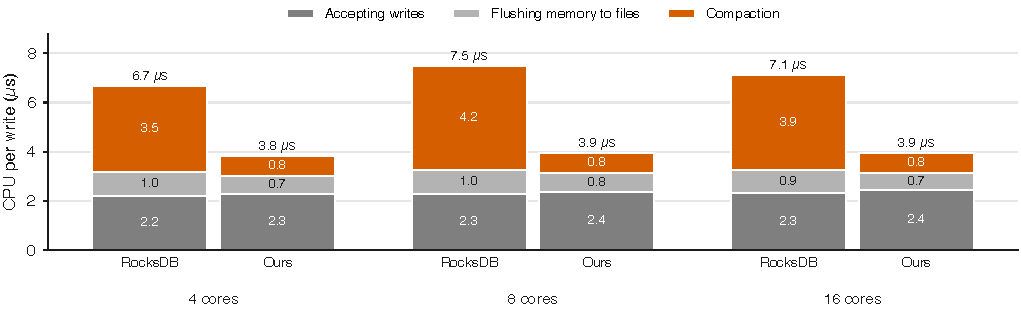
\includegraphics[width=0.8\textwidth]{fig39_cpu_per_write.pdf}
  \caption{CPU per write, split by job: accepting writes, flushing memory to files and
  compaction. RocksDB and whole-compaction offload, each tuned for 4, 8 and 16 cores; LZ4,
  128\,B values, data in memory, median of 5 runs. In RocksDB, compaction is the largest
  share; after offload, accepting writes is.}
  \label{fig:cpu-split}
\end{figure*}

\paragraph{Where the CPU goes.} Figure~\ref{fig:cpu-split} splits RocksDB's CPU per write
by job when it writes as fast as it can. Compaction takes 3.5--5.5\,\textmu s per write,
flushing 1.0 and accepting the write 2.3. Compaction is therefore the part worth moving, and
it is the part earlier accelerator designs target.

\subsection{What earlier designs leave on the CPU}
\label{sec:motivation}

Earlier accelerator designs fall into two families (Table~\ref{tab:designs}). Their published
numbers come from LevelDB, X-Engine and key-value-separated stores, on different hardware.
To compare them with each other and with whole-compaction offload, we rebuilt each family
inside the same RocksDB. The rebuilds are stage-placement rebuilds, not reproductions of the
original systems: they measure where each family puts the work, with the same kernels, so each runs our GPU code for the steps that family offloads and
RocksDB's own CPU code for the others. The rebuilds are generous: input decompression runs on
four parallel threads rather than one, and LUDA's CPU-assisted sort is replaced by our GPU
merge. Every rebuild passes the same check against unmodified RocksDB as our design. The
construction and fairness rules were registered before the runs.

\begin{table}[t]
  \caption{What each design runs on the accelerator, and how we rebuilt it.}
  \label{tab:designs}
  \small
  \begin{tabular}{p{0.24\columnwidth}p{0.33\columnwidth}p{0.33\columnwidth}}
    \toprule
    Design (stands in for) & On the accelerator & Left on the CPU in our rebuild \\
    \midrule
    Sort/merge (gLSM~\cite{glsm2024}, gParaKV~\cite{gparakv2025}) & unpack, sort, merge,
      drop hidden versions & decompression, iterator, block building, compression,
      checksums \\
    Pipeline (LUDA~\cite{luda2020}, MSST'24~\cite{zhou2024msst}, FPGA~\cite{fpga2020}) &
      unpack, sort, merge, deletions, block building, filter hashes & decompression,
      compression, checksums \\
    This work & steps 1--4 and Bloom-filter hashing & file cuts, index, metadata, file
      writing \\
    \bottomrule
  \end{tabular}
\end{table}

\begin{table}[t]
  \caption{Compaction CPU-seconds per GiB of input for one compaction, median of 3 warm runs
  (lower is better). Earlier designs rebuilt in the same RocksDB; one RTX A6000. A separate
campaign from Figure~\ref{fig:compaction}, whose absolute values differ; compare within the
table.}
  \label{tab:prior-cpu}
  \small
  \begin{tabular}{lrrrr}
    \toprule
    Workload & RocksDB & Sort/merge & Pipeline & Ours \\
    \midrule
    32\,B values, LZ4   & 16.93 & 12.40 &  6.08 & \textbf{2.31} \\
    128\,B values, LZ4  & 11.04 &  8.21 &  5.44 & \textbf{2.10} \\
    1\,KB values, LZ4   &  5.69 &  4.58 &  3.92 & \textbf{1.96} \\
    128\,B values, ZSTD & 20.46 & 17.32 & 14.15 & \textbf{2.19} \\
    128\,B values, none &  5.10 &  3.44 &  1.81 & \textbf{1.80} \\
    \bottomrule
  \end{tabular}
\end{table}

Table~\ref{tab:prior-cpu} shows the result. The pipeline design, the stronger family, still
uses 49\% of RocksDB's compaction CPU with LZ4 (5.44 of 11.04 CPU-s per GiB for 128-byte
values) and 69\% with ZSTD. Our design uses 2.0--6.5$\times$ less than the pipeline design
when blocks are compressed. With compression off, the pipeline design and ours are equal (1.81
and 1.80), so what the earlier designs leave behind is the codec. Checksums cost no measurable
CPU in this comparison. % data/summary.md; RELATED-WORK.md 1

\takeaway{Earlier accelerator designs leave block compression and decompression on the
CPU, and that is half to two-thirds of the compaction CPU they set out to remove.}

\subsection{One database leaves the GPU mostly idle}
\label{sec:motivation-idle}

Offloading the codec makes a GPU fast enough to replace many cores: eight concurrent
compactions run at 1.42\,GiB/s of LZ4 input on one RTX A6000 using 2.0 host cores, the
compaction rate of 15 RocksDB cores (18 for ZSTD). But a database rarely needs that much
compaction. One database of 4 cores writing as fast as it can kept a remote GPU busy 19\% of
the time in our registered measurement (Section~\ref{sec:eval-sharing}), and 27--42\% on the
same machine. % M5 Y1; multiplex/analyze.py M1 GPU busy at N = 1

Table~\ref{tab:cost-throughput} prices this. We price each GPU as the cheapest AWS instance GPU
with at least its memory and bandwidth (the RTX A6000 as an L40S at \$1.68 an hour) and CPU
cores at the per-core price of a general-purpose instance (\texttt{prices.json}). These are costs of compaction throughput, not of writes; Section~\ref{sec:eval-cost}
prices whole writes. A GPU dedicated to one database costs 1.39$\times$ as much per GiB/s of
compaction as RocksDB's cores.
The same GPU shared by enough work to keep its engines busy costs 0.89$\times$, and the remote
service at eight databases 0.83$\times$.

\begin{table}[t]
  \caption{Cost of compaction throughput (128\,B values, LZ4): dollars per hour for each GiB/s
  of compaction input. Derived by \texttt{cost\_model.py} from archived runs.}
  \label{tab:cost-throughput}
  \small
  \begin{tabular}{p{0.46\columnwidth}rrr}
    \toprule
    Where compaction runs & GiB/s & \$/h per GiB/s & vs.\ cores \\
    \midrule
    RocksDB, CPU cores (per core, scaled) & 0.094 & 0.945 & 1.00 \\
    GPU dedicated to one database & 1.417 & 1.314 & 1.39 \\
    GPU shared through the service at capacity & 2.418 & 0.843 & 0.89 \\
    Remote service, 8 databases (RTX PRO 6000) & 4.304 & 0.781 & 0.83 \\
    \bottomrule
  \end{tabular}
\end{table}

\takeaway{A GPU that compacts for one database is mostly idle and dearer than the cores it
replaces; it is cheaper only when several databases share it.}

% ------------------------------------------------------------------------------------------
\section{Design Overview}
\label{sec:overview}

\begin{figure}[t]
  \centering
  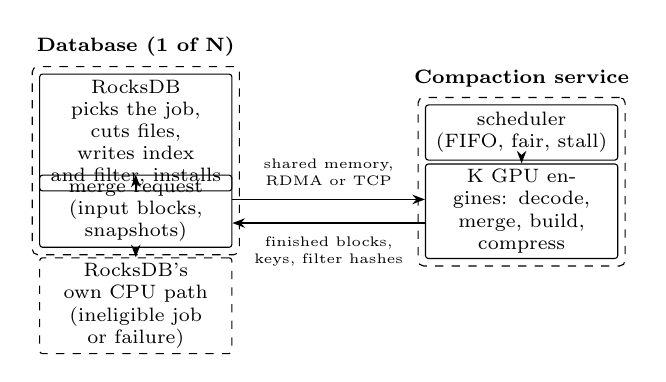
\begin{tikzpicture}[
      font=\scriptsize,
      box/.style={draw, rounded corners=1pt, align=center, inner sep=2pt, text width=23mm,
                  minimum height=7mm},
      grp/.style={draw, dashed, rounded corners=2pt, inner sep=2.5pt},
      arr/.style={-{Stealth[length=1.6mm]}, semithick},
      note/.style={font=\tiny, align=center}]
    \node[box] (rdb) at (0, 0) {RocksDB picks the job,\\cuts files, writes index\\and filter, installs};
    \node[box] (req) at (0, -10mm) {merge request\\(input blocks, snapshots)};
    \node[box] (sch) at (49mm, 0) {scheduler\\(FIFO, fair, stall)};
    \node[box] (eng) at (49mm, -10mm) {K GPU engines: decode,\\merge, build, compress};
    \node[grp, fit=(rdb)(req), label={[font=\scriptsize\bfseries]above:Database (1 of N)}] {};
    \node[grp, fit=(sch)(eng), label={[font=\scriptsize\bfseries]above:Compaction service}] {};
    \draw[arr] (rdb) -- (req);
    \draw[arr] (sch) -- (eng);
    \draw[arr] ([yshift=1.5mm]req.east) -- node[note, above=0.5mm] {shared memory,\\RDMA or TCP}
      ([yshift=1.5mm]eng.west);
    \draw[arr] ([yshift=-1.5mm]eng.west) -- node[note, below=0.5mm] {finished blocks,\\keys, filter hashes}
      ([yshift=-1.5mm]req.east);
    \node[box, dashed] (cpu) at (0, -22mm) {RocksDB's own CPU path\\(ineligible job or failure)};
    \draw[arr, dashed] (req) -- (cpu);
  \end{tikzpicture}
  \caption{Architecture. RocksDB keeps every decision that shapes the tree; a shared service
  turns each merge request into finished, compressed blocks.}
  \label{fig:architecture}
\end{figure}

Figure~\ref{fig:architecture} shows the architecture. The two findings of
Section~\ref{sec:background} set four goals.

\begin{itemize}
  \item \textbf{G1, RocksDB shapes the tree.} RocksDB picks every compaction, decides where
        output files end, writes indexes and filter metadata, and installs the result. The
        accelerator returns blocks, never files, so the file format and the rules that
        shape the tree do not change.
  \item \textbf{G2, the whole compaction.} Steps 1--4 run on the GPU, including the codec,
        which is what earlier designs leave on the CPU (Section~\ref{sec:motivation}).
  \item \textbf{G3, never lose a compaction.} A job the GPU cannot take, or a failed call,
        runs on RocksDB's own code in the database process.
  \item \textbf{G4, one GPU for many databases.} The GPU belongs to a service rather than to
        a database, so its cost is divided by the databases it serves, wherever they run
        (Section~\ref{sec:motivation-idle}).
\end{itemize}

\noindent Three things are out of scope: the SSD-to-GPU data path that recent
work optimises~\cite{zhou2024msst,gpcomp2025,gclcomp2025}, key-value
separation~\cite{gparakv2025}, and isolating tenants' use of shared memory bandwidth.

\paragraph{Life of a compaction.} RocksDB picks a compaction and splits it into
subcompactions as usual. For each subcompaction it sends one merge request: the list of input
data blocks with their bytes, the snapshots, the levels involved and the output block
options. The request goes to a GPU engine in the same process, or to the compaction service,
which queues it until an engine is free. The engine returns finished, compressed and
checksummed blocks with two boundary keys per block and the keys' filter hashes. RocksDB
appends the blocks to output files, cutting files where its own rules say, and builds each
file's index and filter from them. If the request is ineligible or the call fails, RocksDB
compacts the same input on the CPU.

% ------------------------------------------------------------------------------------------
\section{Whole-Compaction Offload}
\label{sec:offload}

\subsection{Interface}
A version-locked patch to RocksDB~11.8 adds a table option,\linebreak \texttt{CompactionBlockTransform}.
With no transform set, RocksDB runs unchanged. For each eligible subcompaction, RocksDB lists
every data block of every input file within the subcompaction's bounds and calls the
transform with one \texttt{CompactionMergeRequest}. A transform may run on a GPU in the same
process, on the CPU (the reference implementation we check the GPU against), or remotely.

\subsection{The GPU pipeline}
One engine, with its own CUDA stream and buffers, runs a job in five phases.
\begin{enumerate}
  \item \textbf{Read and decode.} Input blocks are read into pinned memory by parallel
        threads. On the device, block checksums (CRC32C) are verified and blocks are decoded
        with nvCOMP~\cite{nvcomp} LZ4 or ZSTD, one batched call per codec.
  \item \textbf{Merge.} Every restart interval is parsed in parallel. Entries arrive as
        sorted runs (each level-0 file, and each deeper level), so the runs are merged
        pairwise with a merge-path kernel rather than sorted.
  \item \textbf{Drop.} Entries hidden by a newer version of the same user key, with no
        snapshot between the two versions, are dropped, exactly as RocksDB's \texttt{CompactionIterator} does.
        Deletions are dropped when the key cannot exist below the output level; sequence
        numbers are zeroed at the bottommost level as RocksDB does.
  \item \textbf{Build.} Blocks are cut by replaying \texttt{BlockBuilder}'s size estimate and
        flush policy (a block also ends every 2{,}048 entries, so cutting runs in parallel),
        then key-delta encoded with restart arrays.
  \item \textbf{Compress and seal.} Blocks are compressed with nvCOMP LZ4 or ZSTD in RocksDB's
        block layout, kept compressed only within RocksDB's ratio limit, and given a masked
        CRC32C (one warp per block). The engine computes the filter hash of every key.
\end{enumerate}
Only the finished blocks, two boundary keys per block and the filter hashes return to the
host. On an RTX A6000, eight concurrent subcompactions reach about 1.4\,GiB/s of LZ4 input and
0.9\,GiB/s of ZSTD input, limited mainly by nvCOMP compression.

\subsection{Keeping RocksDB in charge of the tree}
RocksDB's own file-cut decision (\texttt{ShouldStopBefore}, refactored to take a key) runs at
each block's first key, and files are cut only between user keys. Each run of blocks that
stays in one file is appended with one write: RocksDB fills each block's trailer (compression type and checksum) into a gap left by the
GPU and adds
index entries as it goes. RocksDB chooses each filter's size, probe count and metadata; the
GPU sets its bits from the hashes. Job statistics are accounted so that RocksDB's own
record-count verification holds.

\subsection{Eligibility and fallback}
A subcompaction is offloaded when it has no merge operator, compaction filter, blob files or
range tombstones, uses the bytewise comparator, and reads format-6 files with CRC32C and LZ4,
ZSTD or no compression, with internal keys of at most 512 bytes. Building blocks on the GPU
further requires default table options and a whole-key Bloom or Ribbon filter. Anything else
runs on RocksDB's own iterators, and the reason is recorded. A failed GPU call falls back to the
CPU for that job; a checksum or parse error fails the compaction as RocksDB would.

\subsection{Correctness}
\label{sec:correct}
Every single-compaction run hashes every stored version (user key, sequence number, type,
value) and the results of 200{,}000 point lookups, which exercise the GPU-built Bloom filters
and indexes, and compares them with unmodified RocksDB. Every whole-database run checks each
read as it happens and every key and value at the end. The GPU code passes NVIDIA's
\texttt{compute-sanitizer} memory, race and synchronisation checks. The output is logically
identical to RocksDB's, not byte-identical: GPU ZSTD uses nvCOMP's compression level, so
compressed bytes differ while the decompressed data is the same.

% ------------------------------------------------------------------------------------------
\section{The Shared Compaction Service}
\label{sec:service}

Section~\ref{sec:offload} removes the codec from the CPU, which makes one GPU worth
15--18 cores; Section~\ref{sec:motivation-idle} shows one database cannot use that. Because a
merge request carries its own input and the reply is finished blocks, a GPU can serve
databases whose files it never sees. The service turns this into a shared resource.

\paragraph{One context, K engines.} One server process owns the GPU and serves every database
from one CUDA context and K engines; a database process keeps none. Each job needs 11--17
times its compressed input in GPU memory, so K is bounded by memory. We choose K by a rule
registered in advance: replaying 138 recorded compaction requests from 16 clients, the
fewest engines within 95\% of the best throughput. On a 48\,GB RTX A6000 that is K\,=\,4
(2.42\,GiB/s of input, 31\,GiB of GPU memory); 8 engines exceed the GPU's memory and fall to
2.13\,GiB/s.

\paragraph{Scheduling.} Each request carries its tenant and two hints: whether its writers
were stalled when the job was built, and level~0's size against its slowdown trigger. When an
engine frees, the scheduler picks the next job by policy: \emph{fifo} (arrival order),
\emph{fair} (start-time fair queuing over tenants, charged by input bytes) or \emph{stall}
(jobs that unblock writers first, then fair order). An optional memory budget starts a job
only when the estimates of running jobs fit.

\paragraph{Out of GPU memory.} A job that fails to allocate GPU memory is not failed. Idle
engines free their cached buffers, and the job runs again after another job finishes, up to
8 times, keeping its place in the policy order.

\paragraph{Transports.} A request carries all of its input blocks, so the service needs no
shared file system. On one machine, requests and replies stay in shared memory that the client
owns and passes to the server once. Between machines, RDMA moves requests with one-sided
writes into pre-registered buffers taken from a capped pool shared by a process's
connections, costing the client about 0.012 CPU-seconds per GiB against about 0.7 over TCP.
TCP is used where RDMA is unavailable, for example in a public cloud.

\paragraph{Failures.} A call that fails or times out falls back to RocksDB's CPU path for that
job (G3). Because a request is self-contained, a client may also retry it on a new connection.
On SIGTERM the server can drain: it refuses new merges with \emph{Busy}, which clients retry
elsewhere, and finishes the running ones before exiting. A replica behind a load balancer can
therefore be replaced without CPU fallbacks.

% ------------------------------------------------------------------------------------------
\section{Implementation}
\label{sec:impl}
The RocksDB patch is applied at build time to a pinned RocksDB~11.8 commit; its public
interface is a 270-line header. The GPU engine is about 3{,}900 lines of CUDA using nvCOMP~5.3.
The CPU reference merge and the scheduler add about 1{,}100 lines of C++, and the service and
its transports (shared memory, TCP, and RDMA over \texttt{libibverbs} and
\texttt{librdmacm}) about 2{,}700. The benchmarks, the experiment drivers, the registered
hypotheses and every run's raw records will be released with the paper.
\todo{Artifact URL after review.}

% ------------------------------------------------------------------------------------------
\section{Evaluation}
\label{sec:eval}

We answer six questions, in the order of the argument:
\textbf{Q1}~How much faster and cheaper in CPU is one compaction?
\textbf{Q2}~What does the whole database gain, against RocksDB and earlier designs?
\textbf{Q3}~Does it help real workloads, and does it hurt reads?
\textbf{Q4}~What remains when a drive is the bottleneck?
\textbf{Q5}~How many databases can share one GPU, locally or over the network?
\textbf{Q6}~What does it cost?

\subsection{Methodology}
\label{sec:method}
\paragraph{Hardware.}
\begin{itemize}
  \item \emph{Server~1:} four Xeon Gold 5220, an RTX A6000 (48\,GB) and a SATA SSD.
  \item \emph{Server~2:} a Xeon Silver 4210R, an RTX PRO 6000 Blackwell Max-Q (96\,GB) and an
        NVMe SSD.
  \item \emph{Database machine:} 96 cores on two NUMA nodes, connected to server~2 by
        100\,Gb/s RoCE (ConnectX-6 Dx, 92\,Gb/s measured).
\end{itemize}

\paragraph{Baselines.} RocksDB~11.8 is the baseline in every run. RocksDB and our design are
each tuned for each core count by the same search over threads, subcompactions, pipelined
writes and background jobs; both keep RocksDB's default compaction triggers; each database gets whole physical cores within one NUMA node. Earlier designs are
rebuilt in the same RocksDB (Section~\ref{sec:motivation}).

\paragraph{Regime.} Unless stated otherwise: 50\,M keys, 16\,B uniform keys, 128\,B values about
2:1 compressible (half random, half a repeating pattern), writes in batches of 100, the
write-ahead log off, and data in memory (\texttt{/dev/shm}). This makes compaction the
bottleneck. We report drive-bound runs, runs with the log on, YCSB~\cite{cooper2010ycsb} and
published production workload models~\cite{cao2020} separately.

\paragraph{Protocol.}
\begin{itemize}
  \item Fixed-duration runs (30\,s warm-up plus 120\,s, or 2 plus 5 minutes) in random order,
        with medians of 3--5 runs.
  \item Throughput is counted in the writing window and, where compaction is left over, to its
        end.
  \item Hypotheses, thresholds and decision rules were registered before the runs, and every
        number comes from archived runs.
\end{itemize}

\subsection{Q1: One compaction}
\label{sec:eval-compaction}
\begin{figure}[t]
  \centering
  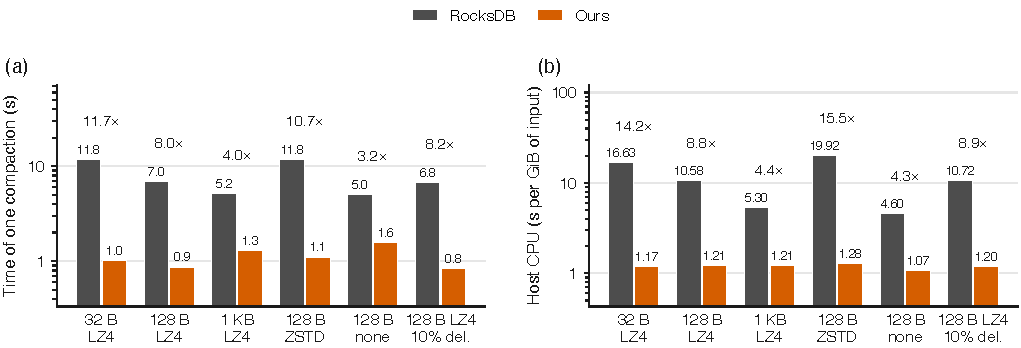
\includegraphics[width=\columnwidth]{fig17_v3_compaction.pdf}
  \caption{One compaction (0.6--0.7\,GiB of input), RocksDB against GPU offload: time and CPU
  per GiB. Median of 3 runs, log scale.}
  \label{fig:compaction}
\end{figure}
Figure~\ref{fig:compaction} shows one compaction on server~1. The offload is
8.0--11.7$\times$ faster and uses 8.8--15.5$\times$ less CPU for 32--128\,B values,
4.0$\times$ / 4.4$\times$ at 1\,KB, and 3.2$\times$ / 4.3$\times$ without compression. Its CPU
stays near 1.2\,CPU-s per GiB whatever the values, because the host only reads input files and
writes output. Table~\ref{tab:prior-cpu} places the earlier designs between RocksDB and ours.

\takeaway{One compaction is 8--12$\times$ faster with 9--16$\times$ less CPU for small
compressed values; the gain shrinks to 3--4$\times$ for 1\,KB values or no compression.}

\subsection{Q2: Whole database}
\label{sec:eval-db}
\begin{figure}[t]
  \centering
  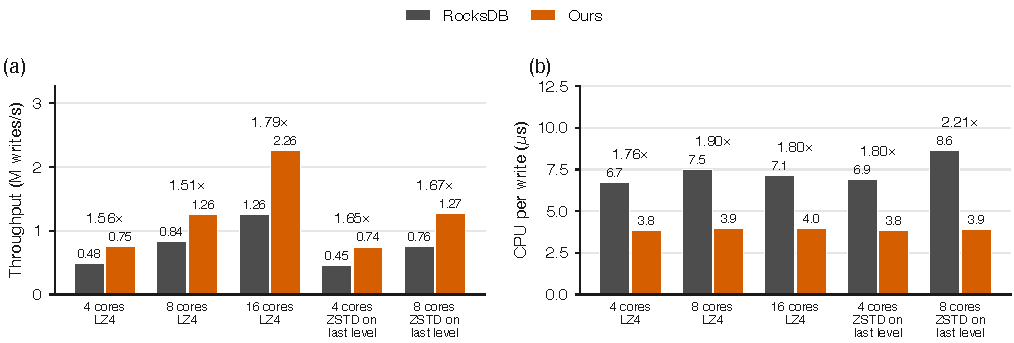
\includegraphics[width=\columnwidth]{fig19_v3_database.pdf}
  \caption{Whole database, default regime, tuned settings, median of 5 runs.}
  \label{fig:database}
\end{figure}

\paragraph{Throughput and CPU.} With LZ4, the database accepts 1.56$\times$, 1.51$\times$ and
1.79$\times$ more writes at 4, 8 and 16 cores (Figure~\ref{fig:database}), and uses
1.76--1.90$\times$ less CPU per write. With ZSTD on the last level the gains are
1.65--1.67$\times$. Compaction CPU per write falls from 3.5--5.5\,\textmu s to 0.8\,\textmu s,
while the cost of accepting a write is unchanged at 2.3\,\textmu s; that cost now bounds
throughput (Figure~\ref{fig:cpu-split}). RocksDB slowed its writers for up to 6\% of the time;
ours never did. RocksDB also left 11--69\,s of compaction after 5 minutes of writing, against
1.3--2.6\,s for ours; counting that compaction, the gains are 1.55--1.86$\times$.

\paragraph{Tail latency at a fixed load.} At 50\%, 70\% and 90\% of RocksDB's maximum
throughput, 99.9th-percentile write latency is 1.75$\times$, 3.8$\times$ and 9.6$\times$ lower.
We had registered 2.5$\times$ at 50\%, which was not met; the 90\% point was added after the
registration.

\paragraph{A machine shared with other work.} Benchmarks usually get the whole machine; real
databases do not. Following LUDA~\cite{luda2020}, a separate
process burns a fixed share of each of the database's 4 cores. With 40\% of each core taken,
our design accepts 2.17$\times$ RocksDB's writes; with 80\%, 2.48$\times$, against 1.80$\times$
with no competing process. RocksDB loses 11\% of its throughput going from 40\% to 80\% and
ours nothing measurable, because its compaction is not on those cores.
% FULL-RESULTS 6, contention campaign, median of 3

\paragraph{Against earlier designs.} With 4 cores and default settings, the sort/merge,
pipeline and whole-compaction designs accept 1.14$\times$, 1.41$\times$ and 1.75$\times$
RocksDB's writes with LZ4, and 1.16$\times$, 1.17$\times$ and 2.27$\times$ with ZSTD. Tuned,
they reach 498k, 592k and 756k writes/s with LZ4. With compression off they reach
0.98$\times$, 1.34$\times$ and 1.40$\times$: the pipeline design and ours are close, as in
Table~\ref{tab:prior-cpu}. gParaKV's and LUDA's own code run on different stores, so we
report them separately and do not compare against them here.

\todo{E3: 500\,M keys (about 70\,GB, larger than memory) on NVMe with a block cache, once
archived.}

\takeaway{When compaction is the CPU bottleneck, the database takes 1.5--1.8$\times$ more
writes for about half the CPU per write, and more when other work competes for its cores.
What remains is the cost of accepting writes, which offload does not touch.}

\subsection{Q3: Real workloads and reads}
\label{sec:eval-workloads}

\paragraph{YCSB.} Table~\ref{tab:ycsb} shows YCSB~\cite{cooper2010ycsb} on 4 cores. Read-heavy
work (B) is unchanged, within 5\% in throughput and equal in read latency, which we had
registered as a no-harm check. Where compaction is busy (A and F), throughput rises
1.24--1.67$\times$, and read-modify-write's p99 read latency halves, because reads no longer
compete with compaction for the same cores.

\begin{table}[t]
  \caption{YCSB on 4 cores: operations per second and p99 read latency, median of 3 runs.}
  \label{tab:ycsb}
  \small
  \setlength{\tabcolsep}{3pt}
  \begin{tabular}{lrrrrr}
    \toprule
    & \multicolumn{3}{c}{Ops/s} & \multicolumn{2}{c}{p99 read (ms)} \\
    Workload & RocksDB & Ours & Gain & RocksDB & Ours \\
    \midrule
    B (95\% reads), unif. & 272k & 277k & 1.02$\times$ & 0.025 & 0.025 \\
    B, Zipfian              & 498k & 522k & 1.05$\times$ & 0.019 & 0.018 \\
    A (50\% reads), unif. & 190k & 273k & 1.44$\times$ & 0.029 & 0.027 \\
    A, Zipfian              & 314k & 388k & 1.24$\times$ & 0.022 & 0.020 \\
    F (read-mod.-write), unif. & 103k & 172k & 1.67$\times$ & 0.147 & 0.074 \\
    F, Zipfian              & 178k & 230k & 1.31$\times$ & 0.090 & 0.051 \\
    \bottomrule
  \end{tabular}
\end{table}
% FULL-RESULTS 5, ycsb campaign

\todo{E1: YCSB A--F (adding C, D and E with scans), uniform and Zipfian, at 8 and 16 cores.}

\paragraph{Production workload models.} Meta's ZippyDB model~\cite{cao2020}, run through
RocksDB's MixGraph, gains 1.05$\times$ and 1.10$\times$ at 8 and 16 cores with its 85\% reads,
and 1.34$\times$ and 1.70$\times$ in a write-heavy variant. Models of a stream-processing state
store, storage metadata and a time series with deletions gain 1.38--1.77$\times$, two of them
with the write-ahead log on.

\todo{E2: a real application on RocksDB (Kvrocks) with our RocksDB build, once feasible and
archived.}

\takeaway{The gain follows how much compaction a workload creates: read-heavy work is
unchanged, write-heavy work gains up to 1.7$\times$, and no workload we measured had slower reads.}

\subsection{Q4: When the drive is the bottleneck}
\label{sec:storage}
\begin{figure}[t]
  \centering
  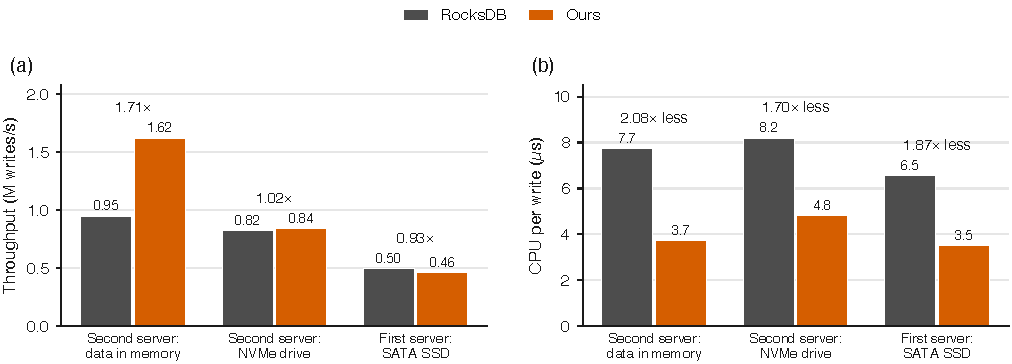
\includegraphics[width=\columnwidth]{fig33_storage.pdf}
  \caption{Throughput and CPU per write in memory, on NVMe (server~2) and on a SATA SSD
  (server~1), 8 cores.}
  \label{fig:storage}
\end{figure}
On a drive, the drive limits both systems (Figure~\ref{fig:storage}). Throughput is unchanged:
1.02$\times$ on NVMe, and 0.93$\times$ and 1.04$\times$ on SATA. The CPU saving remains: CPU per
write is 1.70$\times$ lower on NVMe and 1.87--2.0$\times$ lower on SATA. At 630k writes/s on
NVMe, p99 write latency is 17\,ms against 503\,ms. Ours keeps the NVMe drive 89--90\% busy
against 55\%, because it writes 5.5 bytes per user byte against 4.0. The main cause is that its faster
compactions start with fewer level-0 files (Section~\ref{sec:limits}).

\takeaway{When the drive is the limit, throughput is equal and the gain is CPU (1.7--2.0$\times$
less per write) and tail latency.}

\subsection{Q5: One GPU, many databases}
\label{sec:eval-sharing}

\paragraph{One database, remote GPU.} Sending each compaction over RDMA to server~2's GPU
makes it 4.0--6.5$\times$ faster than RocksDB on the database machine, which spends
5.6--11$\times$ less CPU on it. Of the 0.9--1.1\,s a remote compaction takes, about 0.2\,s is
on the network and 0.2--0.35\,s on the GPU; the rest is reading and writing files on the
database machine. The whole database, with 4 cores, accepts 802k writes/s against RocksDB's
459k (1.75$\times$) with 2.04$\times$ less CPU per write on the database machine, or
1.84$\times$ less including the GPU server's CPU. A remote CPU server saves the same
database-machine CPU, but each compaction takes about twice as long as in RocksDB.

\todo{E5: the same eight databases served by a pool of remote CPU cores instead of the GPU
(CaaS-LSM style): cores needed to match, and cost.}

\paragraph{Capacity of one service.} We registered this experiment (M5) with three
predictions before running it:
\begin{itemize}
  \item \emph{Setup:} N databases of 4 cores on the database machine share one service on
        server~2 (4 cores, K engines, fair scheduling) over RDMA. RocksDB runs on the same
        cores.
  \item \emph{Protocol:} 3 repetitions in shuffled order, with GPU utilisation sampled every
        second. All 27 trials verified every key and had no CPU fallback and no out-of-memory
        failure.
\end{itemize}
Table~\ref{tab:capacity} and Figure~\ref{fig:capacity} show the results.

\begin{table}[t]
  \caption{One remote service shared by N databases of 4 cores (M5). Writes/s per database in
  the window and counted to the end of the leftover compaction; leftover compaction after
  writing stops; GPU utilisation during writing; worst p99.9 write latency. Median of 3.}
  \label{tab:capacity}
  \small
  \setlength{\tabcolsep}{3.5pt}
  \begin{tabular}{lrrrrrr}
    \toprule
     & N & Window & With leftover & Leftover & GPU & p99.9 \\
    \midrule
    RocksDB        & 1 & 475k & 465k & 6.3\,s & -- & 10.5\,ms \\
    RocksDB        & 8 & 402k & 394k & 8.5\,s & -- & 11.0\,ms \\
    Service, K\,=\,4 & 1 & 918k & 914k & 0.9\,s & 19\% & 8.1\,ms \\
    Service, K\,=\,4 & 4 & 872k & 865k & 1.7\,s & 72\% & 8.9\,ms \\
    Service, K\,=\,4 & 6 & 830k & 816k & 3.5\,s & 96\% & 8.9\,ms \\
    Service, K\,=\,4 & 8 & 837k & 783k & 10.9\,s & 98\% & 7.6\,ms \\
    Service, K\,=\,8 & 8 & 834k & 784k & 10.0\,s & 96\% & 7.9\,ms \\
    \bottomrule
  \end{tabular}
\end{table}

The registered predictions and their outcomes:
\begin{itemize}
  \item \emph{The GPU is mostly idle for one database} (at most 40\%): supported, 19\%.
  \item \emph{Eight databases each get at least 1.8$\times$ RocksDB's writes, with no CPU
        fallback:} supported. Each gets 783k against 394k (1.99$\times$), counting the
        leftover compaction, and keeps 86\% of its throughput when alone. This replicates an
        earlier registered run (2.01$\times$).
  \item \emph{Eight engines give at least 10\% more than four at N\,=\,8:} not supported
        (1.00$\times$). From six databases the GPU itself is 93--98\% busy, so more engines have
        nothing to use.
\end{itemize}

By the registered capacity rule (the largest N within 80\% of one database, with no
fallback), one service handled at least 8 databases, the most that fit in the database
machine's memory. The GPU saturates at about 6 databases. From 6 to 8, total writes in the
window rise from 4.98M to 6.70M per second. Part of the rise is compaction deferred past the
window (the leftover grows from 3.5 to 10.9\,s); counting it, the total still rises from
4.90M to 6.26M. These are 5-minute runs, so they show what the service sustains over that
period, not an indefinite steady state near saturation. Tail latency stays below RocksDB's at every N,
and the slowest database reaches 0.95 of the fastest at N\,=\,8. The service used 1.8 of its 4
cores.

\paragraph{Sharing on one machine.} Three ways to share server~1's GPU (Table~\ref{tab:local}):
each database process using the GPU itself, the same through CUDA MPS~\cite{cudamps}, and the
service over shared memory. Throughput is similar: with four databases of 8 cores, MPS reached
1{,}149k writes/s per database and the service 1{,}121k (fair) or 1{,}144k (FIFO). A repeat
of the largest cases found the difference within run-to-run variation. Two things differ.
\begin{itemize}
  \item \emph{CPU fallbacks:} separate processes and MPS fall back to the CPU when GPU memory
        runs out; the service never did, in 66 registered runs.
  \item \emph{Fairness:} the slowest database reaches 0.87 of the fastest with the service,
        against 0.73 with MPS.
\end{itemize}

\begin{table}[t]
  \caption{Databases sharing server~1's GPU (RTX A6000), main runs: writes/s per database,
  slowest/fastest database, CPU fallbacks over 3 runs, and worst p99.9 write latency.}
  \label{tab:local}
  \small
  \setlength{\tabcolsep}{3pt}
  \begin{tabular}{llrrrr}
    \toprule
    DBs$\times$cores & Arm & Writes/s & Slow/fast & Fallbacks & p99.9 \\
    \midrule
    4$\times$8 & RocksDB       &   811k & 0.94 &   0 & 28.3\,ms \\
    4$\times$8 & Separate      & 1{,}107k & 0.78 &  38 & 30.4\,ms \\
    4$\times$8 & MPS           & 1{,}149k & 0.73 &   1 & 28.3\,ms \\
    4$\times$8 & Service, fair & 1{,}121k & 0.87 &   0 & 18.9\,ms \\
    6$\times$4 & RocksDB       &   441k & 0.81 &   0 & 19.9\,ms \\
    6$\times$4 & Separate      &   517k & 0.71 & 158 & 25.2\,ms \\
    6$\times$4 & MPS           &   593k & 0.78 & 107 & 24.1\,ms \\
    6$\times$4 & Service, fair &   490k & 0.97 &   0 & 24.1\,ms \\
    \bottomrule
  \end{tabular}
\end{table}

\paragraph{Isolation.} One heavy database (unlimited writes) and three light ones (363k
writes/s each, open loop) share the service with one engine. Two of the light databases share
a NUMA node with the heavy database and the service. We registered that fair or stall-first
scheduling would keep the light databases' p99.9 within 1.5$\times$ of running alone. It was
not met: their worst p99.9 was 4.31$\times$ (FIFO), 4.46$\times$ (fair) and 4.15$\times$
(stall-first) their solo 13.6\,ms. Every light database kept its rate. Follow-up runs
(exploratory) point away from the queue: the light database on the other NUMA node stayed
within 1.1--1.3$\times$, and with four engines the light databases waited only 51\,ms per job
yet their latency was 5.85$\times$. Without the service, with the same placement, it was
1.69$\times$. The slowdown therefore comes from the service's work on that node; whether
through memory bandwidth or CPU, we did not measure.

\todo{E4: stop the service during a run with four databases; fallback to the CPU, throughput
over time and recovery.}

\takeaway{One GPU serves at least eight remote databases, each at about twice RocksDB's
writes, with no compaction falling back to the CPU. On one machine the service matches CUDA
MPS in throughput but never falls back and is fairer; it does not isolate tenants on its own
NUMA node.}

\subsection{Q6: Cost}
\label{sec:eval-cost}
\begin{itemize}
  \item \emph{Pricing:} as in Section~\ref{sec:motivation-idle}. Server~2's GPU is priced as
        the same card on AWS (\$3.01 an hour), and the service's 4 cores are included.
  \item \emph{Dedicated GPU:} with one database per GPU, ours is cheaper per write only beyond
        RocksDB's highest rate. 16 cores with a GPU reach 2.26M writes/s, 23\% cheaper per
        write than RocksDB's 1.60M on 32 cores (break-even \$2.61 an hour). At the same rate,
        RocksDB is cheaper unless the GPU costs at most \$0.71 an hour.
  \item \emph{Shared service:} at 8 databases, \$0.258 against RocksDB's \$0.246 per billion
        writes (5\% more). Compaction is cheaper per GiB/s (Table~\ref{tab:cost-throughput}),
        but a write also pays for the database's cores and the service's host. It breaks even at a GPU price of \$2.73 an hour, \$1.92 at 6
        databases and \$1.31 at 4.
  \item \emph{Cheaper GPUs:} a cheaper card with at least the 31\,GiB the service's engines
        use would make the service cheaper per write than RocksDB, but we did not measure one.
        We report break-even prices so that readers can apply their own.
\end{itemize}
% cost_model.py; multiplex/analyze.py (M5 break-even); FULL-RESULTS 7 and 11

\todo{E6: energy per write counted to the end of the leftover compaction.}

\takeaway{A GPU is the cheaper way to reach write rates RocksDB cannot. Shared by eight
databases it costs about the same per write as RocksDB (5\% more at the measured card's
price) and is cheaper below \$2.73 an hour.}

% ------------------------------------------------------------------------------------------
\section{Discussion and Limitations}
\label{sec:limits}
\begin{itemize}
  \item \textbf{Regime.} The largest gains need compaction to be the CPU bottleneck. Our
        headline regime (log off, batched writes, data in memory, values compressing 2:1)
        makes it so. With the log on and one write at a time the gain is 1.34$\times$; on a
        drive it is none, though CPU per write still falls 1.7--2.0$\times$. Production
        ZippyDB data compresses 4.5:1~\cite{cao2020}; we did not measure such data.
  \item \textbf{Cost.} Shared at the measured card's price, the service costs 5\% more per
        write than RocksDB. Its case rests on capacity and consolidation, and on cheaper
        GPUs, for which we report break-even prices rather than measurements.
  \item \textbf{Isolation.} The service does not isolate tenants on its NUMA node
        (Section~\ref{sec:eval-sharing}). CaaS-LSM's global scheduling~\cite{caaslsm2024} is
        the yardstick here.
  \item \textbf{Write amplification.} It is about 1.4$\times$ higher than RocksDB's, all in
        compaction output. With the same trigger, our faster compactions start with fewer
        level-0 files (5.6 against 9.4 on NVMe), so each entry is rewritten more often.
        Raising our level-0 trigger from 4 to 24 lowers write amplification in memory from
        6.36 to 3.09; about 13\% of the difference is unexplained. Part of our gain in
        stalls and latency may therefore come from compacting earlier rather than from the
        GPU; a comparison at matched level-0 depth would separate the two.
  \item \textbf{Coverage.} We do not offload merge operators, compaction filters, range
        tombstones or blob files, which fall back to RocksDB. Without compression our design
        has no advantage over the pipeline design.
  \item \textbf{Scope.} Two GPU models, one RocksDB version, one RDMA machine pair and one
        database machine; we make no energy claim yet.
  \item \textbf{Missed predictions.} Registered predictions not met: tail latency at 50\%
        load; tenant isolation; eight engines over four; the service beating MPS on one
        machine; its cost per write with four local databases; and two replication
        predictions. All are listed with the registration.
\end{itemize}
% PREREGISTRATION.md lists every registered hypothesis and outcome.
% TODO(cloud): add the registered Kubernetes runs (PREREGISTRATION.md, "Cloud") once archived.

% ------------------------------------------------------------------------------------------
\section{Related Work}
\label{sec:related}

\paragraph{Accelerated compaction.}
\begin{itemize}
  \item \emph{LUDA}~\cite{luda2020} moves LevelDB's sort, merge, block building and checksums
        to a GPU, and leaves compression as future work.
  \item \emph{gLSM}~\cite{glsm2024} and \emph{gParaKV}~\cite{gparakv2025} sort and merge on the
        GPU in key-value-separated stores. Separating values compacts fewer bytes, which is
        complementary to our work. gParaKV is faster than RocksDB under its own driver, and
        we do not claim otherwise.
  \item \emph{An FPGA design}~\cite{fpga2020} offloads the merge pipeline in X-Engine and
        reports up to 23\% more throughput.
  \item \emph{The NVMe data path:} the MSST'24 design~\cite{zhou2024msst},
        GPComp~\cite{gpcomp2025} and GCLComp~\cite{gclcomp2025} optimise moving data between
        NVMe and the GPU, which matters most where our design gains least, on a drive.
  \item \emph{A concurrent prototype}~\cite{reevalgpcomp} re-evaluates GPComp-style
        compaction against RocksDB's multi-threaded compaction.
\end{itemize}
Each of these is evaluated on its own store and hardware. We rebuild them in one RocksDB,
which shows what they leave on the CPU. To our knowledge, none offloads block compression or
shares a GPU across databases.
\todo{Confirm for GPComp and GCLComp from their full texts.}

\paragraph{Compaction as a service and disaggregated LSM-trees.}
\begin{itemize}
  \item \emph{Compaction on other machines:} CaaS-LSM~\cite{caaslsm2024} runs RocksDB's
        compaction as a stateless remote CPU service, with global priority scheduling and
        error handling. Nova-LSM~\cite{novalsm2021} offloads compaction to storage nodes over
        RDMA, and dLSM~\cite{dlsm2023} compacts near the data on disaggregated memory.
  \item \emph{Compacting once for replicas:} Tebis~\cite{tebis2022} and
        RubbleDB~\cite{rubbledb2023} compact on the primary and ship the result to replicas.
\end{itemize}
Our service follows CaaS-LSM in making compaction a disaggregated resource. It differs in
using a GPU and in what it ships: the input blocks rather than access to shared files. None of
these systems uses a GPU.

\paragraph{Making compaction cheaper or smoother on the CPU.} SILK~\cite{silk2019} schedules
compaction I/O to avoid latency spikes, and ADOC~\cite{adoc2023} tunes threads and batch sizes
to avoid write stalls. Sarkar et al.~\cite{sarkar2021} map the design space of compaction
strategies, and Spooky~\cite{spooky2022} chooses compaction granularity to lower space and
write amplification. These change \emph{when} and \emph{what} RocksDB compacts; we change
\emph{where} it runs, and our offload leaves those decisions to RocksDB, so the two compose.

% ------------------------------------------------------------------------------------------
\section{Conclusion}
\label{sec:conclusion}
Earlier accelerator designs leave block compression on the CPU, and that is most of what they
set out to remove. Offloading the whole compaction, codec included, lets one GPU do the
compaction work of 15--18 cores while RocksDB keeps control of its tree. One database leaves
such a GPU mostly idle, so GPU compaction pays as a shared service: eight databases sharing
one remote GPU each get twice RocksDB's writes on the same cores over 5-minute runs, with no compaction
falling back to the CPU. What remains is to isolate tenants and to measure cheaper GPUs, on
which the service's cost advantage depends.

\bibliographystyle{ACM-Reference-Format}
\bibliography{refs}

\end{document}
